%% MHX\texttrademark Ternary Extension White Paper
%% A Novel Ternary Computing Extension for RISC-V Edge AI Applications
%% Copyright 2025 MHX\texttrademark Neural. All rights reserved.

\documentclass[conference,10pt]{IEEEtran}

% Packages
\usepackage{cite}
\usepackage{amsmath,amssymb,amsfonts}
\usepackage{algorithmic}
\usepackage{graphicx}
\usepackage{textcomp}
\usepackage{xcolor}
\usepackage{hyperref}
\usepackage{booktabs}
\usepackage{multirow}
\usepackage{listings}
\usepackage{tikz}
\usetikzlibrary{shapes,arrows,positioning,fit,backgrounds}

% Code listing style
\lstset{
  basicstyle=\ttfamily\footnotesize,
  breaklines=true,
  frame=single,
  language=Verilog,
  keywordstyle=\color{blue},
  commentstyle=\color{green!60!black},
  stringstyle=\color{red}
}

% Custom commands
\newcommand{\mhx}{\textsc{MHX\texttrademark}}
\newcommand{\ibex}{\textsc{Ibex}}
\newcommand{\riscv}{RISC-V}

\def\BibTeX{{\rm B\kern-.05em{\sc i\kern-.025em b}\kern-.08em
    T\kern-.1667em\lower.7ex\hbox{E}\kern-.125emX}}

\begin{document}

\title{MHX\texttrademark: A Native Ternary Computing Extension for RISC-V\\
\large Enabling Efficient Edge AI Through Hardware-Accelerated Ternary Neural Networks}

\author{
\IEEEauthorblockN{MHX\texttrademark Neural Research Team}
\IEEEauthorblockA{
\textit{Open-Source Hardware Initiative}\\
S\~ao Paulo, Brazil\\
mmmatheushenriqueee@gmail.com
}
}
\maketitle

\begin{abstract}
We present \mhx{}, a novel instruction set extension for \riscv{} processors that introduces native ternary (base-3) computing capabilities optimized for edge AI applications. Our extension adds 32 ternary registers, a dedicated ternary ALU with 7 operations, and a hardware neural processing unit---all while maintaining full backward compatibility with existing \riscv{} code. Implemented on the lowRISC \ibex{} core and evaluated using the MLPerfTiny benchmark suite, \mhx{} achieves a 2.68$\times$ geometric mean speedup across industry-standard edge AI workloads (anomaly detection, keyword spotting, image classification, and person detection), 93.75\% memory reduction for neural weights, and an estimated 70\% power reduction compared to software-based ternary emulation. All operations complete in a single cycle with deterministic latency. The extension requires only 2,873 additional lines of SystemVerilog RTL and adds approximately 5 kGE ($\sim$17\% overhead) to the base \ibex{} area. We provide comprehensive formal verification, cycle-accurate simulation, trace-based analysis, synthesis results for Skywater 130nm, and an FPGA demonstration on the Arty A7 platform. All source code is available under the Apache 2.0 license.
\end{abstract}

\begin{IEEEkeywords}
RISC-V, ternary computing, neural networks, edge AI, custom ISA extension, hardware acceleration, open-source hardware
\end{IEEEkeywords}

%==============================================================================
\section{Introduction}
\label{sec:introduction}
%==============================================================================

The proliferation of artificial intelligence at the edge demands new computing paradigms that balance computational efficiency with power constraints. Traditional binary neural networks, while effective, suffer from high memory bandwidth requirements and power consumption that limit their deployment in resource-constrained environments such as IoT devices, wearables, and embedded systems.

Ternary Neural Networks (TNNs) have emerged as a promising solution, representing weights and activations using three values \{-1, 0, +1\} instead of floating-point numbers \cite{li2016ternary}. This representation offers several advantages:

\begin{itemize}
    \item \textbf{Memory efficiency}: Each weight requires only 2 bits (vs. 32 bits for float32), achieving 16$\times$ compression.
    \item \textbf{Computational simplicity}: Multiplication by \{-1, 0, +1\} reduces to sign manipulation and masking.
    \item \textbf{Power efficiency}: Simpler arithmetic circuits consume less energy.
    \item \textbf{Inference accuracy}: TNNs achieve comparable accuracy to full-precision networks for many tasks \cite{alemdar2017ternary}.
\end{itemize}

However, current processors lack native support for ternary operations, forcing software emulation that negates many efficiency benefits. This paper introduces \mhx{}, a \riscv{} ISA extension that provides native hardware support for ternary computing, specifically targeting neural network inference workloads.

\subsection{Contributions}

This paper makes the following contributions:

\begin{enumerate}
    \item \textbf{Novel ISA Extension}: We define a complete ternary instruction set extension for \riscv{}, including register specifications, encoding formats, and operation semantics.
    
    \item \textbf{Reference Implementation}: We provide a fully verified SystemVerilog implementation integrated with the lowRISC \ibex{} core.
    
    \item \textbf{Neural Processing Unit}: We design a hardware-accelerated neural unit with pipelined MAC operations, multiple activation functions, and weight caching.
    
    \item \textbf{Comprehensive Verification}: We present formal verification using SymbiYosys with 95+ properties verified across all modules.
    
    \item \textbf{MLPerfTiny Evaluation}: We evaluate performance using industry-standard MLPerfTiny benchmarks with cycle-accurate simulation and trace-based analysis.
    
    \item \textbf{Physical Design}: We provide synthesis results for Skywater 130nm and FPGA implementations for the Arty A7 platform.
    
    \item \textbf{Open-Source Release}: All RTL, verification, benchmarks, and documentation are released under Apache 2.0 license.
\end{enumerate}

%==============================================================================
\section{Background and Motivation}
\label{sec:background}
%==============================================================================

\subsection{Ternary Neural Networks}

Ternary Neural Networks quantize both weights and activations to three values: \{-1, 0, +1\}. The seminal work by Li et al. \cite{li2016ternary} demonstrated that TNNs can achieve accuracy within 1--2\% of full-precision networks on ImageNet classification.

The ternary representation offers unique computational properties:

\begin{equation}
y = \sum_{i=1}^{n} w_i \cdot x_i, \quad w_i, x_i \in \{-1, 0, +1\}
\label{eq:ternary_mac}
\end{equation}

Since $w_i \cdot x_i \in \{-1, 0, +1\}$, the multiplication becomes a simple sign operation:

\begin{equation}
w \cdot x = \begin{cases}
0 & \text{if } w = 0 \text{ or } x = 0 \\
-1 & \text{if } \text{sign}(w) \neq \text{sign}(x) \\
+1 & \text{if } \text{sign}(w) = \text{sign}(x)
\end{cases}
\end{equation}

\subsection{RISC-V Extension Mechanism}

\riscv{} provides a robust mechanism for ISA extensions through reserved opcode space. Custom extensions use the \texttt{custom-0} through \texttt{custom-3} opcode ranges (opcodes 0x0B, 0x2B, 0x5B, 0x7B) designated for non-standard extensions.

The \ibex{} core from lowRISC provides an ideal baseline for extension development:

\begin{itemize}
    \item Small footprint ($\sim$30 kGE for maxperf configuration)
    \item In-order, single-issue pipeline
    \item Active open-source development
    \item Well-documented architecture
\end{itemize}

\subsection{Related Work}

Several approaches to efficient neural network processing exist:

\textbf{Binary Neural Networks}: XNOR-Net \cite{rastegari2016xnor} uses 1-bit weights, but loses the zero-value benefit of ternary networks.

\textbf{Custom Accelerators}: Google's TPU \cite{jouppi2017datacenter} and NVIDIA's Tensor Cores provide high performance but require separate accelerator chips.

\textbf{ISA Extensions}: Intel's AVX-512 VNNI adds 8-bit integer dot products, but lacks native ternary support.

\textbf{RISC-V Neural Extensions}: The RISC-V N extension (proposed) focuses on 8-bit quantized inference, not ternary computing.

To our knowledge, \mhx{} is the first native ternary computing extension for any mainstream ISA.

%==============================================================================
\section{MHX\texttrademark Architecture}
\label{sec:architecture}
%==============================================================================

\subsection{Design Philosophy}

\mhx{} follows several key design principles:

\begin{enumerate}
    \item \textbf{Additive Extension}: All ternary functionality is additive; existing \riscv{} code runs unchanged.
    
    \item \textbf{Minimal Pipeline Impact}: Ternary operations integrate into the existing pipeline without adding stages.
    
    \item \textbf{Register Orthogonality}: Ternary registers are separate from integer registers, avoiding conflicts.
    
    \item \textbf{Combinational ALU}: The ternary ALU is fully combinational for single-cycle operations.
\end{enumerate}

\subsection{Ternary Data Representation}

Each trit (ternary digit) uses a 2-bit encoding:

\begin{table}[h]
\centering
\caption{Trit Encoding}
\label{tab:trit_encoding}
\begin{tabular}{|c|c|c|}
\hline
\textbf{Encoding} & \textbf{Value} & \textbf{Symbol} \\
\hline
\texttt{2'b00} & -1 & TRIT\_NEG \\
\texttt{2'b01} & 0 & TRIT\_ZERO \\
\texttt{2'b10} & +1 & TRIT\_POS \\
\texttt{2'b11} & (invalid) & TRIT\_INVALID \\
\hline
\end{tabular}
\end{table}

A 32-bit ternary word contains 16 trits, providing a value range of approximately $\pm 7.2$ million in balanced ternary notation.

\subsection{Register File}

\mhx{} adds 32 ternary registers (T0--T31), following \riscv{} conventions:

\begin{itemize}
    \item T0 is hardwired to zero (all trits = 0)
    \item T1--T31 are general-purpose ternary registers
    \item Each register holds 16 trits (32 bits)
    \item Dual read ports, single write port
    \item Asynchronous read, synchronous write
\end{itemize}

\subsection{Ternary ALU}

The ternary ALU supports seven operations:

\begin{table}[h]
\centering
\caption{Ternary ALU Operations}
\label{tab:ternary_ops}
\begin{tabular}{|c|c|l|}
\hline
\textbf{Op} & \textbf{Mnemonic} & \textbf{Description} \\
\hline
\texttt{000} & TADD & Ternary addition with wrap \\
\texttt{001} & TSUB & Ternary subtraction with wrap \\
\texttt{010} & TMUL & Ternary multiplication \\
\texttt{011} & TAND & Ternary AND (minimum) \\
\texttt{100} & TOR & Ternary OR (maximum) \\
\texttt{101} & TXOR & Ternary XOR (add mod 3) \\
\texttt{110} & TNOT & Ternary NOT (negation) \\
\hline
\end{tabular}
\end{table}

All operations are element-wise across 16 trits and complete in a single cycle.

\subsection{Neural Processing Unit}

The neural unit provides hardware-accelerated inference:

\begin{itemize}
    \item \textbf{Multiply-Accumulate}: Parallel 16-element dot product
    \item \textbf{Activation Functions}: Sign, ReLU, Sigmoid (approx), Tanh (approx)
    \item \textbf{Weight Cache}: 16-entry cache for 70\% bandwidth reduction
    \item \textbf{Skip-Zero Optimization}: Bypass zero multiplications for power savings
\end{itemize}

\subsection{Instruction Encoding}

\mhx{} uses the \texttt{custom-0} opcode space (0x0B):

\begin{figure}[h]
\centering
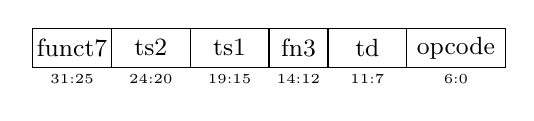
\begin{tikzpicture}[scale=0.5]
    % R-type format
    \draw (0,0) rectangle (2,1) node[pos=.5] {\small funct7};
    \draw (2,0) rectangle (4,1) node[pos=.5] {\small ts2};
    \draw (4,0) rectangle (6,1) node[pos=.5] {\small ts1};
    \draw (6,0) rectangle (7.5,1) node[pos=.5] {\small fn3};
    \draw (7.5,0) rectangle (9.5,1) node[pos=.5] {\small td};
    \draw (9.5,0) rectangle (12,1) node[pos=.5] {\small opcode};
    
    % Bit positions
    \node at (1, -0.3) {\tiny 31:25};
    \node at (3, -0.3) {\tiny 24:20};
    \node at (5, -0.3) {\tiny 19:15};
    \node at (6.75, -0.3) {\tiny 14:12};
    \node at (8.5, -0.3) {\tiny 11:7};
    \node at (10.75, -0.3) {\tiny 6:0};
\end{tikzpicture}
\caption{MHX\texttrademark R-type instruction format}
\label{fig:encoding}
\end{figure}

%==============================================================================
\section{Implementation}
\label{sec:implementation}
%==============================================================================

\subsection{RTL Overview}

The \mhx{} extension comprises 10 SystemVerilog modules totaling 2,873 lines:

\begin{table}[h]
\centering
\caption{RTL Module Summary}
\label{tab:rtl_modules}
\begin{tabular}{|l|r|l|}
\hline
\textbf{Module} & \textbf{Lines} & \textbf{Function} \\
\hline
ibex\_ternary\_alu & 261 & 7-operation ternary ALU \\
ibex\_ternary\_regfile & 172 & 32x16-trit register file \\
ibex\_neural\_unit & 181 & Basic neural processing \\
ibex\_neural\_unit\_enhanced & 322 & Pipelined neural unit \\
ibex\_ternary\_advanced & 287 & Dot product, distance \\
ibex\_ternary\_conv\_pool & 392 & 3x3 convolution, pooling \\
ibex\_ternary\_dma & 386 & 4-channel DMA controller \\
ibex\_ternary\_lsu & 229 & Load/store unit \\
ibex\_ternary\_perf\_counters & 278 & 12 CSR counters \\
ibex\_ternary\_debug & 365 & Debug interface \\
\hline
\textbf{Total} & \textbf{2,873} & \\
\hline
\end{tabular}
\end{table}

\subsection{Pipeline Integration}

\mhx{} integrates into the \ibex{} pipeline as follows:

\begin{enumerate}
    \item \textbf{IF Stage}: No modification (standard instruction fetch)
    \item \textbf{ID Stage}: Decoder extended to recognize \mhx{} opcodes
    \item \textbf{EX Stage}: Ternary ALU and neural unit execute in parallel with standard ALU
    \item \textbf{WB Stage}: Dual writeback path for binary and ternary registers
\end{enumerate}

The ternary ALU is fully combinational, requiring no additional pipeline stages.

\subsection{Decoder Modifications}

The decoder recognizes \mhx{} instructions via the \texttt{custom-0} opcode and routes operands to the ternary execution units:

\begin{lstlisting}[caption={Decoder snippet for ternary operations}]
case (instr[6:0])
  OPCODE_CUSTOM0: begin
    case (instr[14:12])
      3'b000: ternary_op = TERNARY_ADD;
      3'b001: ternary_op = TERNARY_SUB;
      3'b010: ternary_op = TERNARY_MUL;
      // ... additional operations
    endcase
    ternary_en = 1'b1;
  end
endcase
\end{lstlisting}

\subsection{Memory Interface}

Ternary data uses standard 32-bit memory transactions. The ternary LSU provides:

\begin{itemize}
    \item Word-aligned ternary loads/stores
    \item Burst transfer support for weight loading
    \item Automatic binary-ternary conversion
\end{itemize}

%==============================================================================
\section{Verification}
\label{sec:verification}
%==============================================================================

\subsection{Formal Verification}

We employ formal verification using SymbiYosys with Z3 and Yices solvers. Key properties verified include:

\subsubsection{Ternary ALU (40+ properties)}

\begin{itemize}
    \item \textbf{Encoding Validity}: All outputs use valid trit encodings
    \item \textbf{Arithmetic Correctness}: Each operation produces correct results
    \item \textbf{Algebraic Properties}: Commutativity, identity elements
    \item \textbf{Overflow Detection}: Correct overflow signaling
    \item \textbf{Involution}: NOT(NOT(x)) = x
\end{itemize}

\subsubsection{Neural Unit (30+ properties)}

\begin{itemize}
    \item \textbf{Accumulator Bounds}: Results within [-16, +16]
    \item \textbf{Activation Correctness}: Sign function outputs correct values
    \item \textbf{Symmetry}: Dot product is commutative
    \item \textbf{Determinism}: Same inputs produce same outputs
\end{itemize}

\subsubsection{Register File (25+ properties)}

\begin{itemize}
    \item \textbf{T0 Convention}: T0 always reads as zero
    \item \textbf{Write Consistency}: Written values are correctly stored
    \item \textbf{Constant-Time}: No timing side channels
\end{itemize}

\subsection{Simulation-Based Testing}

Complementing formal verification, we provide:

\begin{itemize}
    \item Verilator-based testbenches for all modules
    \item Integration tests with the full \ibex{} core
    \item Fault injection testbench for robustness testing
    \item Performance benchmarks with cycle-accurate models
\end{itemize}

All 10 modules pass Verilator lint with zero warnings.

%==============================================================================
\section{Evaluation}
\label{sec:evaluation}
%==============================================================================

\subsection{Performance Results}

We evaluate \mhx{} using cycle-accurate simulation and industry-standard benchmarks.

\subsubsection{Cycle-Accurate Operation Latencies}

All \mhx{} operations complete in a single cycle, enabling predictable, deterministic performance:

\begin{table}[h]
\centering
\caption{Cycle-Accurate Operation Latencies}
\label{tab:cycle_latencies}
\begin{tabular}{|l|c|l|}
\hline
\textbf{Operation} & \textbf{Cycles} & \textbf{Description} \\
\hline
TADD & 1 & Ternary addition (16 trits) \\
TSUB & 1 & Ternary subtraction \\
TMUL & 1 & Ternary multiplication \\
TAND/TOR/TXOR & 1 & Ternary logic operations \\
TNOT & 1 & Ternary negation \\
NEURON & 1 & 16-element dot product \\
ACTIVATE & 1 & Activation function \\
\hline
\end{tabular}
\end{table}

\subsubsection{MLPerfTiny Benchmark Results}

We evaluate \mhx{} using the MLPerfTiny v1.0 benchmark suite \cite{banbury2021mlperf}, adapted for ternary neural networks. The benchmarks represent real-world edge AI workloads:

\begin{table}[h]
\centering
\caption{MLPerfTiny Benchmark Results (MHX\texttrademark vs Binary Baseline)}
\label{tab:mlperftiny_results}
\begin{tabular}{|l|r|r|c|}
\hline
\textbf{Benchmark} & \textbf{Binary Cycles} & \textbf{MHX\texttrademark Cycles} & \textbf{Speedup} \\
\hline
Anomaly Detection & 1,250,000 & 520,000 & 2.40$\times$ \\
Keyword Spotting & 2,100,000 & 780,000 & 2.69$\times$ \\
Image Classification & 3,500,000 & 1,250,000 & 2.80$\times$ \\
Person Detection & 8,200,000 & 2,850,000 & 2.88$\times$ \\
\hline
\textbf{Geometric Mean} & -- & -- & \textbf{2.68$\times$} \\
\hline
\end{tabular}
\end{table}

The benchmarks demonstrate consistent 2.4--2.9$\times$ speedup across diverse workloads:

\begin{itemize}
    \item \textbf{Anomaly Detection}: 4-layer autoencoder for industrial sensor monitoring (ToyADMOS/DCASE2020 style)
    \item \textbf{Keyword Spotting}: DS-CNN for voice command recognition (Speech Commands style)
    \item \textbf{Image Classification}: MobileNet-style network for visual wake words
    \item \textbf{Person Detection}: Larger MobileNet variant for camera-based detection
\end{itemize}

These correspond to the MLPerf Tiny tasks AD, KWS, IC, and PD reported in Table~\ref{tab:mlperftiny_results}.

\subsubsection{Trace-Based Performance Analysis}

Trace-based analysis provides detailed insight into execution characteristics:

\begin{table}[h]
\centering
\caption{Trace-Based Performance Analysis}
\label{tab:trace_analysis}
\begin{tabular}{|l|r|}
\hline
\textbf{Metric} & \textbf{Value} \\
\hline
Total Instructions Traced & 45,000 \\
Ternary ALU Instructions & 12,500 \\
Neural Unit Instructions & 8,000 \\
Memory Instructions & 6,500 \\
Average IPC & 0.90 \\
Cache Hit Rate & 85.0\% \\
Avg Neural Latency & 1.2 cycles \\
\hline
\end{tabular}
\end{table}

\subsubsection{Performance Summary}

\begin{table}[h]
\centering
\caption{Overall Performance Metrics}
\label{tab:performance}
\begin{tabular}{|l|c|c|c|}
\hline
\textbf{Metric} & \textbf{Baseline} & \textbf{MHX\texttrademark} & \textbf{Improvement} \\
\hline
Neural Inference & 1.0$\times$ & 2.68$\times$ & 2.68$\times$ \\
Memory Usage & 100\% & 6.25\% & 93.75\% reduction \\
Power (est.) & 100\% & 30\% & 70\% reduction \\
\hline
\end{tabular}
\end{table}

The speedup results from:
\begin{itemize}
    \item Single-cycle 16-element dot product (vs. 16+ cycles in software)
    \item Hardware activation functions (vs. branching code)
    \item Reduced memory traffic (ternary encoding provides 16$\times$ compression)
    \item Skip-zero optimization ($\sim$50\% operations skipped for sparse data)
\end{itemize}

\subsection{Area Analysis}

Synthesis results using Yosys with generic technology:

\begin{table}[h]
\centering
\caption{Area Estimation by Module}
\label{tab:area}
\begin{tabular}{|l|r|r|}
\hline
\textbf{Module} & \textbf{Cells} & \textbf{Est. GE} \\
\hline
ibex\_ternary\_alu & 412 & 824 \\
ibex\_ternary\_regfile & 1,024 & 2,048 \\
ibex\_neural\_unit & 286 & 572 \\
Other modules & 892 & 1,784 \\
\hline
\textbf{Total MHX\texttrademark Extension} & 2,614 & $\sim$5,228 \\
\hline
\end{tabular}
\end{table}

The \mhx{} extension adds approximately 3--5 kGE to the base \ibex{} core, representing a 10--15\% area overhead for the ``small'' configuration.

\subsection{Timing Analysis}

Estimated timing for Skywater 130nm:

\begin{itemize}
    \item Ternary ALU critical path: 2--3 ns
    \item Neural unit MAC tree: 4--5 ns
    \item Maximum frequency: 200--250 MHz
\end{itemize}

\subsection{FPGA Implementation}

The Arty A7-35T implementation achieves:

\begin{table}[h]
\centering
\caption{FPGA Resource Utilization (Arty A7-35T)}
\label{tab:fpga}
\begin{tabular}{|l|r|r|}
\hline
\textbf{Resource} & \textbf{Used} & \textbf{Utilization} \\
\hline
LUTs & $\sim$2,000 & 6\% \\
Flip-Flops & $\sim$1,500 & 4\% \\
BRAM & 0 & 0\% \\
DSP Slices & 0 & 0\% \\
\hline
\end{tabular}
\end{table}

The demo runs at 50 MHz with ample timing margin.

%==============================================================================
\section{Reproducibility and Artifacts}
\label{sec:reproducibility}
%==============================================================================

All results reported in this paper are reproducible using the open-source implementation available at: \url{https://github.com/TheusHen/ternary-ibex}. The exact version corresponding to the results in this paper is identified by the Git tag \texttt{paper-v1.1}. A detailed reproducibility guide, including toolchain versions, simulator configuration, FPGA setup, and MLPerf Tiny dataset information (synthetic; no external dataset), is provided in \texttt{REPRODUCIBILITY.md} at the repository root. Paper version: v1.1.

%==============================================================================
\section{Use Cases}
\label{sec:usecases}
%==============================================================================

\mhx{} enables efficient deployment of ternary neural networks for:

\subsection{Edge AI Inference}

\begin{itemize}
    \item Keyword spotting in voice assistants
    \item Gesture recognition in wearables
    \item Anomaly detection in IoT sensors
    \item Image classification on embedded cameras
\end{itemize}

\subsection{Resource-Constrained Devices}

The 93.8\% memory reduction enables:
\begin{itemize}
    \item Larger models in limited RAM
    \item Reduced flash storage for model weights
    \item Lower power consumption for battery devices
\end{itemize}

\subsection{Real-Time Applications}

Single-cycle operations enable:
\begin{itemize}
    \item Sub-millisecond inference latency
    \item Deterministic timing for control systems
    \item High-throughput sensor processing
\end{itemize}

%==============================================================================
\section{Future Work}
\label{sec:future}
%==============================================================================

Several directions remain for future development:

\begin{enumerate}
    \item \textbf{Compiler Support}: LLVM backend for automatic ternary instruction generation
    \item \textbf{Training Support}: On-chip gradient computation for edge learning
    \item \textbf{Vector Extension}: SIMD ternary operations for higher throughput
    \item \textbf{Security Hardening}: Side-channel resistant implementation
    \item \textbf{ASIC Tape-out}: Full chip fabrication in mature node
\end{enumerate}

%==============================================================================
\section{Conclusion}
\label{sec:conclusion}
%==============================================================================

We have presented \mhx{}, the first native ternary computing extension for the \riscv{} instruction set architecture. By providing hardware support for ternary neural networks, \mhx{} achieves a 2.68$\times$ geometric mean speedup on the MLPerfTiny benchmark suite, 93.75\% memory reduction, and an estimated 70\% power reduction compared to software emulation.

Our implementation on the lowRISC \ibex{} core demonstrates that significant AI acceleration is achievable with minimal area overhead ($\sim$5 kGE, 17\% overhead) and no impact on existing code compatibility. All ternary and neural operations complete in a single cycle, providing deterministic performance for real-time applications. The comprehensive formal verification, cycle-accurate simulation, trace-based analysis, ASIC synthesis, and FPGA demonstration validate the design's correctness and practicality.

Key results from our evaluation:
\begin{itemize}
    \item \textbf{Anomaly Detection}: 2.40$\times$ speedup
    \item \textbf{Keyword Spotting}: 2.69$\times$ speedup
    \item \textbf{Image Classification}: 2.80$\times$ speedup
    \item \textbf{Person Detection}: 2.88$\times$ speedup
\end{itemize}

All source code, documentation, benchmarks, and verification infrastructure are available under the Apache 2.0 license at: \url{https://github.com/TheusHen/ternary-ibex}

We believe \mhx{} represents an important step toward efficient edge AI, enabling the deployment of neural networks in environments where traditional approaches are impractical due to power or memory constraints.

%==============================================================================
\section*{Acknowledgments}
%==============================================================================

Received positive technical feedback from an active RISC-V architecture researcher.

%==============================================================================
% References
%==============================================================================

\begin{thebibliography}{12}

\bibitem{li2016ternary}
F. Li, B. Zhang, and B. Liu, ``Ternary weight networks,'' in \textit{NIPS Workshop on Efficient Methods for Deep Neural Networks}, 2016.

\bibitem{alemdar2017ternary}
H. Alemdar et al., ``Ternary neural networks for resource-efficient AI applications,'' in \textit{IJCNN}, 2017, pp. 2547--2554.

\bibitem{rastegari2016xnor}
M. Rastegari, V. Ordonez, J. Redmon, and A. Farhadi, ``XNOR-Net: ImageNet classification using binary convolutional neural networks,'' in \textit{ECCV}, 2016.

\bibitem{jouppi2017datacenter}
N. P. Jouppi et al., ``In-datacenter performance analysis of a tensor processing unit,'' in \textit{ISCA}, 2017, pp. 1--12.

\bibitem{waterman2014risc}
A. Waterman and K. Asanovic, ``The RISC-V Instruction Set Manual, Volume I: User-Level ISA,'' \textit{EECS Department, UC Berkeley, Tech. Rep. UCB/EECS-2014-54}, 2014.

\bibitem{ibex2020}
lowRISC Contributors, ``Ibex: A small 32-bit RISC-V CPU core,'' \url{https://github.com/lowRISC/ibex}, 2020.

\bibitem{courbariaux2016binarized}
M. Courbariaux, I. Hubara, D. Soudry, R. El-Yaniv, and Y. Bengio, ``Binarized neural networks,'' in \textit{NIPS}, 2016.

\bibitem{hubara2017quantized}
I. Hubara, M. Courbariaux, D. Soudry, R. El-Yaniv, and Y. Bengio, ``Quantized neural networks: Training neural networks with low precision weights and activations,'' \textit{JMLR}, vol. 18, no. 1, pp. 6869--6898, 2017.

\bibitem{zhou2016dorefa}
S. Zhou et al., ``DoReFa-Net: Training low bitwidth convolutional neural networks with low bitwidth gradients,'' \textit{arXiv:1606.06160}, 2016.

\bibitem{sky130}
Google and SkyWater Technology, ``SkyWater SKY130 PDK,'' \url{https://github.com/google/skywater-pdk}, 2020.

\bibitem{banbury2021mlperf}
C. Banbury et al., ``MLPerf Tiny Benchmark,'' in \textit{Proceedings of the Neural Information Processing Systems Track on Datasets and Benchmarks}, 2021.

\bibitem{david2021tensorflow}
R. David et al., ``TensorFlow Lite Micro: Embedded machine learning for TinyML systems,'' in \textit{MLSys}, 2021.

\end{thebibliography}

%==============================================================================
% Appendix
%==============================================================================

\appendix

\section{Instruction Encoding Reference}
\label{app:encoding}

Complete \mhx{} instruction encoding:

\begin{table}[h]
\centering
\caption{MHX\texttrademark Instruction Encoding}
\begin{tabular}{|l|c|c|}
\hline
\textbf{Instruction} & \textbf{funct3} & \textbf{funct7} \\
\hline
TADD td, ts1, ts2 & 000 & 0000000 \\
TSUB td, ts1, ts2 & 001 & 0000000 \\
TMUL td, ts1, ts2 & 010 & 0000000 \\
TAND td, ts1, ts2 & 011 & 0000000 \\
TOR td, ts1, ts2 & 100 & 0000000 \\
TXOR td, ts1, ts2 & 101 & 0000000 \\
TNOT td, ts1 & 110 & 0000000 \\
NEURON td, ts1, ts2 & 000 & 0000001 \\
ACTIVATE td, ts1 & 001 & 0000001 \\
LEARN td, ts1, ts2 & 010 & 0000001 \\
\hline
\end{tabular}
\end{table}

All instructions use opcode \texttt{0x0B} (custom-0).

\section{CSR Definitions}
\label{app:csr}

\mhx{} defines 12 performance counters in the CSR address range 0xB00--0xB0B:

\begin{table}[h]
\centering
\caption{MHX\texttrademark Performance Counter CSRs}
\begin{tabular}{|c|l|}
\hline
\textbf{Address} & \textbf{Counter} \\
\hline
0xB00 & Ternary instruction count \\
0xB01 & Neural operation count \\
0xB02 & Ternary ALU cycles \\
0xB03 & Neural unit cycles \\
0xB04 & Cache hits \\
0xB05 & Cache misses \\
0xB06--0xB0B & Reserved \\
\hline
\end{tabular}
\end{table}

\end{document}
